% !TEX TS-program = xelatex
\documentclass[11pt, a4paper]{article}

\usepackage{graphicx}
\usepackage[a4paper, margin=2.5cm]{geometry}
\usepackage{fontspec}
\usepackage[portuguese]{babel}
\babelfont{rm}{Latin Modern Roman}

\usepackage{amsmath}
\usepackage{amssymb}
\usepackage{booktabs}
\usepackage{enumitem}
\setlist[itemize]{label=-}
\usepackage[colorlinks=true, linkcolor=black, citecolor=black, urlcolor=blue]{hyperref}
\usepackage{setspace}

\geometry{top=2.5cm, bottom=2.5cm, left=2.5cm, right=2.5cm}

\begin{document}

\begin{titlepage}
    \centering
    
    % Espaço para logótipo
    \vspace*{1cm}
    
\includegraphics[width=0.8\textwidth]{ISELlogo.png}
    \vspace{1cm}
    
    % Instituição
    {\Large Instituto Superior de Engenharia de Lisboa \par}
    \vspace{0.5cm}
    {\large Licenciatura em Engenharia Física Aplicada \par}
    
    \vfill
    
    % Título
    {\LARGE \textbf{Simulação de Mercados} \par}
    \vspace{0.5cm}
    {\large Física Estatística -- 2º Trabalho \par}
    
    \vfill
    
    % Autores
    \begin{flushleft}
    \textbf{Trabalho realizado por:} \\
    Tiago Bernardo - \textbf{53117} \\
    Gabriel Marques - \textbf{53087}
    \end{flushleft}

    \begin{flushleft}
    \textbf{Docente:} \\
    Prof. Doutor Pedro Patrício
    \end{flushleft}
    
    \vfill
    {\large Novembro de 2026 \par}
    
\end{titlepage}

\newpage
\begin{spacing}{3.5}
    \tableofcontents
\end{spacing}

\newpage
\setcounter{page}{1}

% --- RESUMO ---
\begin{abstract}
Este relatório descreve a aplicação da Mecânica Estatística e da Termodinâmica de Não-Equilíbrio à modelação de sistemas financeiros. Substituindo a clássica hipótese de processos de Markov pelo Movimento Browniano Fracionário (fBM), simulou-se a evolução temporal de um \textit{ensamble} de partículas num espaço sujeito a diferentes dimensões fractais (Expoente de Hurst). O estudo debruça-se sobre a quantificação da agitação térmica (volatilidade), a força advectiva e a memória estocástica através do Deslocamento Quadrático Médio (MSD), da Seta da Entropia de Shannon e do Problema de Fuga de Kramers para estados absorventes.
\end{abstract}

\vspace{0.5cm}

% --- SECÇÕES ---
\section{Introdução}
Na disciplina de Física Estatística \cite{sebenta}, o foco recai habitualmente sobre sistemas em equilíbrio termodinâmico, onde as partículas (como num gás ideal) interagem de forma puramente aleatória, sem memória dos estados anteriores (processos de Markov). Contudo, os mercados financeiros exibem propriedades intrínsecas a sistemas termodinâmicos complexos fora do equilíbrio. A evolução temporal do preço de um ativo pode ser mapeada analogamente à trajetória de uma partícula num banho térmico. 

Como as suposições clássicas de difusão puramente Gaussiana falham em descrever as interações de longo alcance (memória) observadas em sistemas reais, este projeto recorre a teorias mais avançadas de difusão anómala \cite{metzler2014}. O objetivo é generalizar a modelação utilizando um motor de simulação de Monte Carlo. Ao submeter $5\,000$ trajetórias às leis do Movimento Browniano Fracionário, procuramos isolar o impacto do atrito subdifusivo e da inércia superdifusiva na sobrevivência termodinâmica do sistema.

\section{Fundamentação Teórica}

\subsection{Microestados e a Equação de Langevin Generalizada}
A evolução temporal de um ativo $S_t$ é descrita por uma Equação Diferencial Estocástica (SDE) equivalente à Equação de Langevin. Na termodinâmica clássica \cite{sebenta}, a energia cinética média e a agitação das partículas são estritamente proporcionais à temperatura macroscópica. Neste modelo, a volatilidade assume o papel dessa temperatura, e introduz-se a memória espacial no sistema através de um processo de Wiener fracionário $W_t^H$:

\begin{equation}
dS_t = \mu S_t dt + \sigma S_t dW_t^H
\end{equation}

Sob o cálculo estocástico fracionário, Hu e \O{}ksendal \cite{hu2003} deduziram a solução analítica martingala exata desta dinâmica:
\begin{equation}
S_t = S_0 \exp\left(\mu t - \frac{1}{2}\sigma^2 t^{2H} + \sigma W_t^H\right)
\end{equation}

Nesta formulação:
\begin{itemize}
    \item $\mu$ representa o \textbf{Coeficiente de Advecção (Drift)}, a força determinística que atua sobre o sistema.
    \item $\sigma$ é o \textbf{Coeficiente de Difusão}, análogo à temperatura do banho térmico \cite{sebenta}, ditando a amplitude da agitação estocástica diária.
    \item $dW_t^H$ é o ruído térmico correlacionado. Como os conteúdos da sebenta não abrangem a memória fracionária, baseamo-nos nos modelos de difusão anómala de Metzler et al. \cite{metzler2014}, onde o ruído correlacionado é governado pelo Expoente de Hurst ($H \in ]0, 1[$).
\end{itemize}

Os microestados do sistema são definidos pelos retornos logarítmicos:
\begin{equation}
\Delta x = \ln \left( \frac{S_{t+\Delta t}}{S_t} \right)
\end{equation}

A matriz de covariância exata para o cálculo fracionário assenta na relação:
\begin{equation}
\langle W_t^H W_s^H \rangle = \frac{1}{2} \left( t^{2H} + s^{2H} - |t - s|^{2H} \right)
\end{equation}

\subsection{Regimes Termodinâmicos e Dimensões Fractais}
O parâmetro de Hurst ($H$) redefine a geometria do espaço onde as partículas se movem:
\begin{itemize}
    \item \textbf{Subdifusão ($H = 0.25$):} Sistema com autocorrelação negativa. O espaço impõe atrito viscoso severo, criando uma força de reversão elástica.
    \item \textbf{Difusão Normal ($H = 0.50$):} Passeio aleatório markoviano clássico. Ausência de memória térmica ($\langle W_t^{0.5} W_{t+\Delta t}^{0.5} \rangle = 0$).
    \item \textbf{Superdifusão ($H = 0.75$):} Sistema com autocorrelação positiva. Domínio da inércia cinética; o ruído orienta-se favoravelmente numa direção balística.
\end{itemize}

\section{Metodologia e Implementação Computacional}
O estudo recorreu a um \textit{ensamble} de Monte Carlo de $N = 5\,000$ partículas (trajetórias) para um horizonte temporal $T = 1.0$ ano, dividido em 252 passos de interação temporal ($dt$). A simulação foi executada utilizando a fatorização de Cholesky sobre a matriz de covariância do sistema para garantir o rigor das flutuações anómalas. Os parâmetros físicos foram calibrados a partir dos dados com $S_0 = 171.32$, força advectiva $\mu = 0.111\text{ ano}^{-1}$ e agitação térmica $\sigma = 0.138\text{ ano}^{-1}$.

A Figura \ref{fig:base_mercado} ilustra o macroestado base do projeto: a evolução das trajetórias sob difusão normal clássica, evidenciando o cone de dispersão térmica e o valor médio esperado governado pelo \textit{drift}.

\begin{figure}
    \centering
    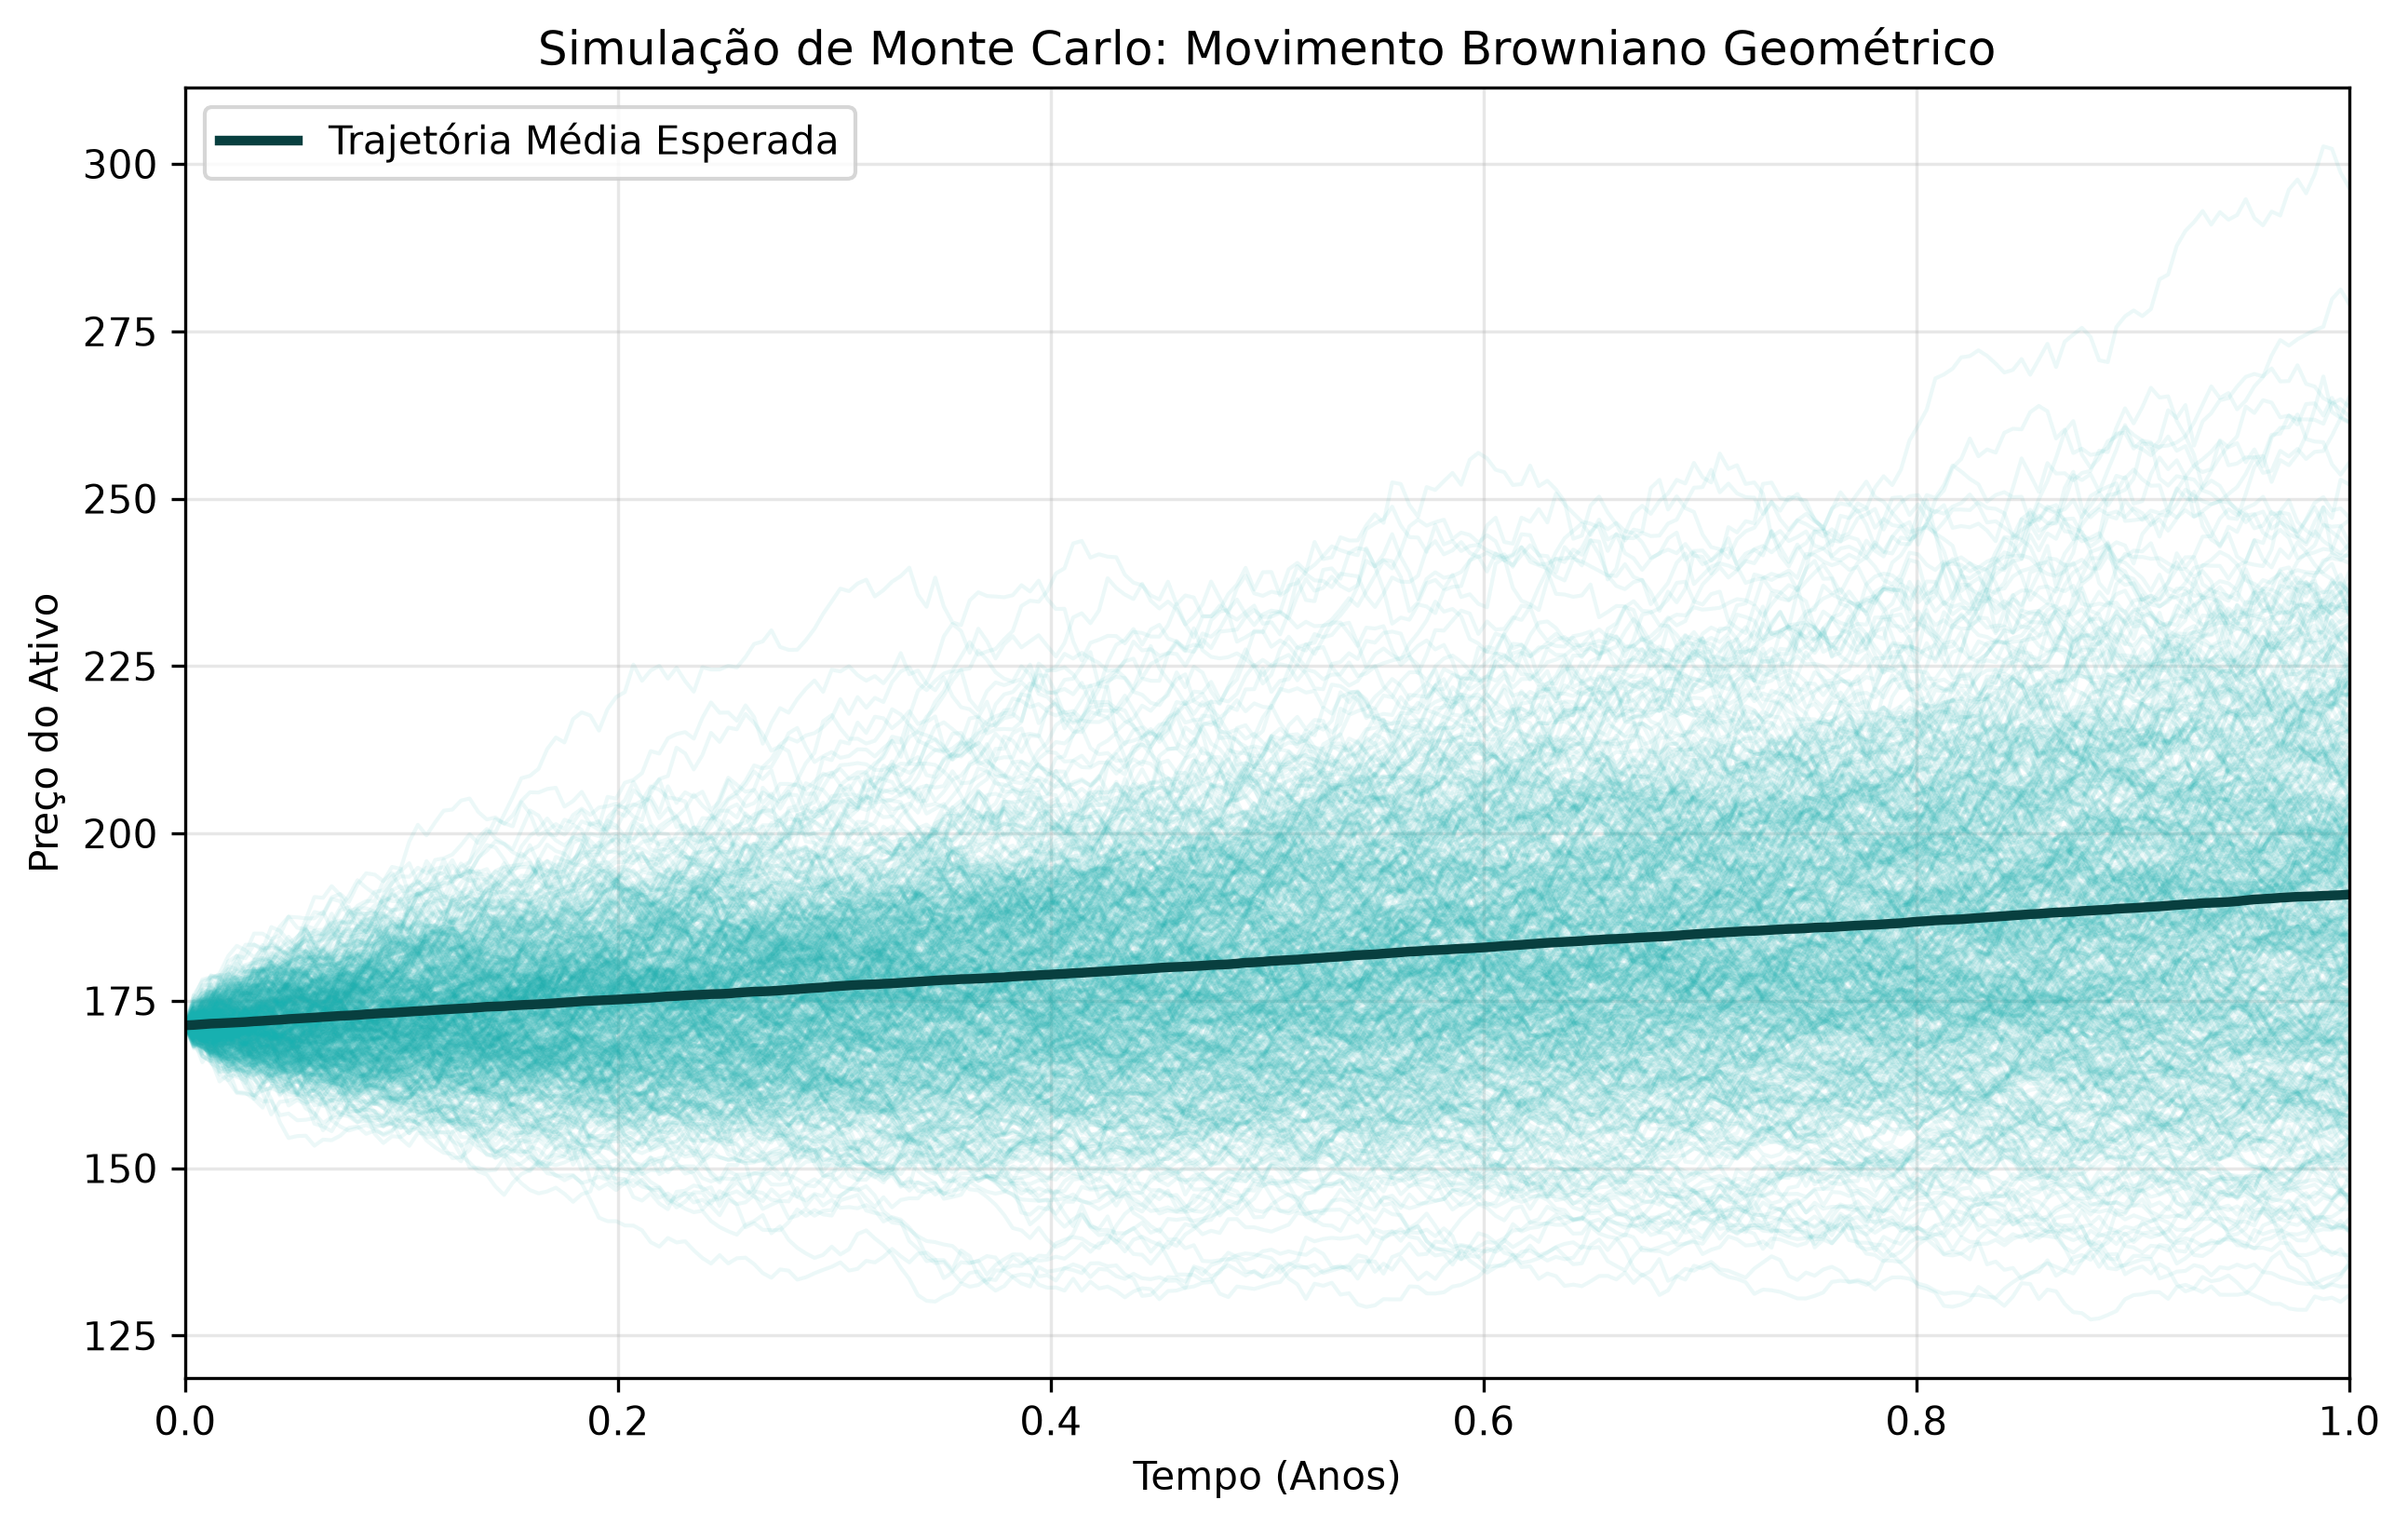
\includegraphics[width=0.85\textwidth]{../Gráficos/01_trajetorias_mercado.png}
    \caption{Simulação base de Monte Carlo: evolução temporal de $500$ trajetórias no regime de difusão normal, com a trajetória média destacada.}
    \label{fig:base_mercado}
\end{figure}

\section{Resultados e Análise Física}

\subsection{O Efeito da Memória na Trajetória (Geometria Espacial)}
Para compreender o impacto da dimensão fractal, isolou-se uma única partícula, submetendo-a à mesma sequência exata de choques térmicos, mas alterando a geometria do espaço (Expoente de Hurst). Como demonstrado na Figura \ref{fig:trajetorias}, a subdifusão atua como uma "mola" de reversão constante, enquanto a superdifusão injeta inércia balística, prolongando as tendências ditadas pela força advectiva.

\begin{figure}
    \centering
    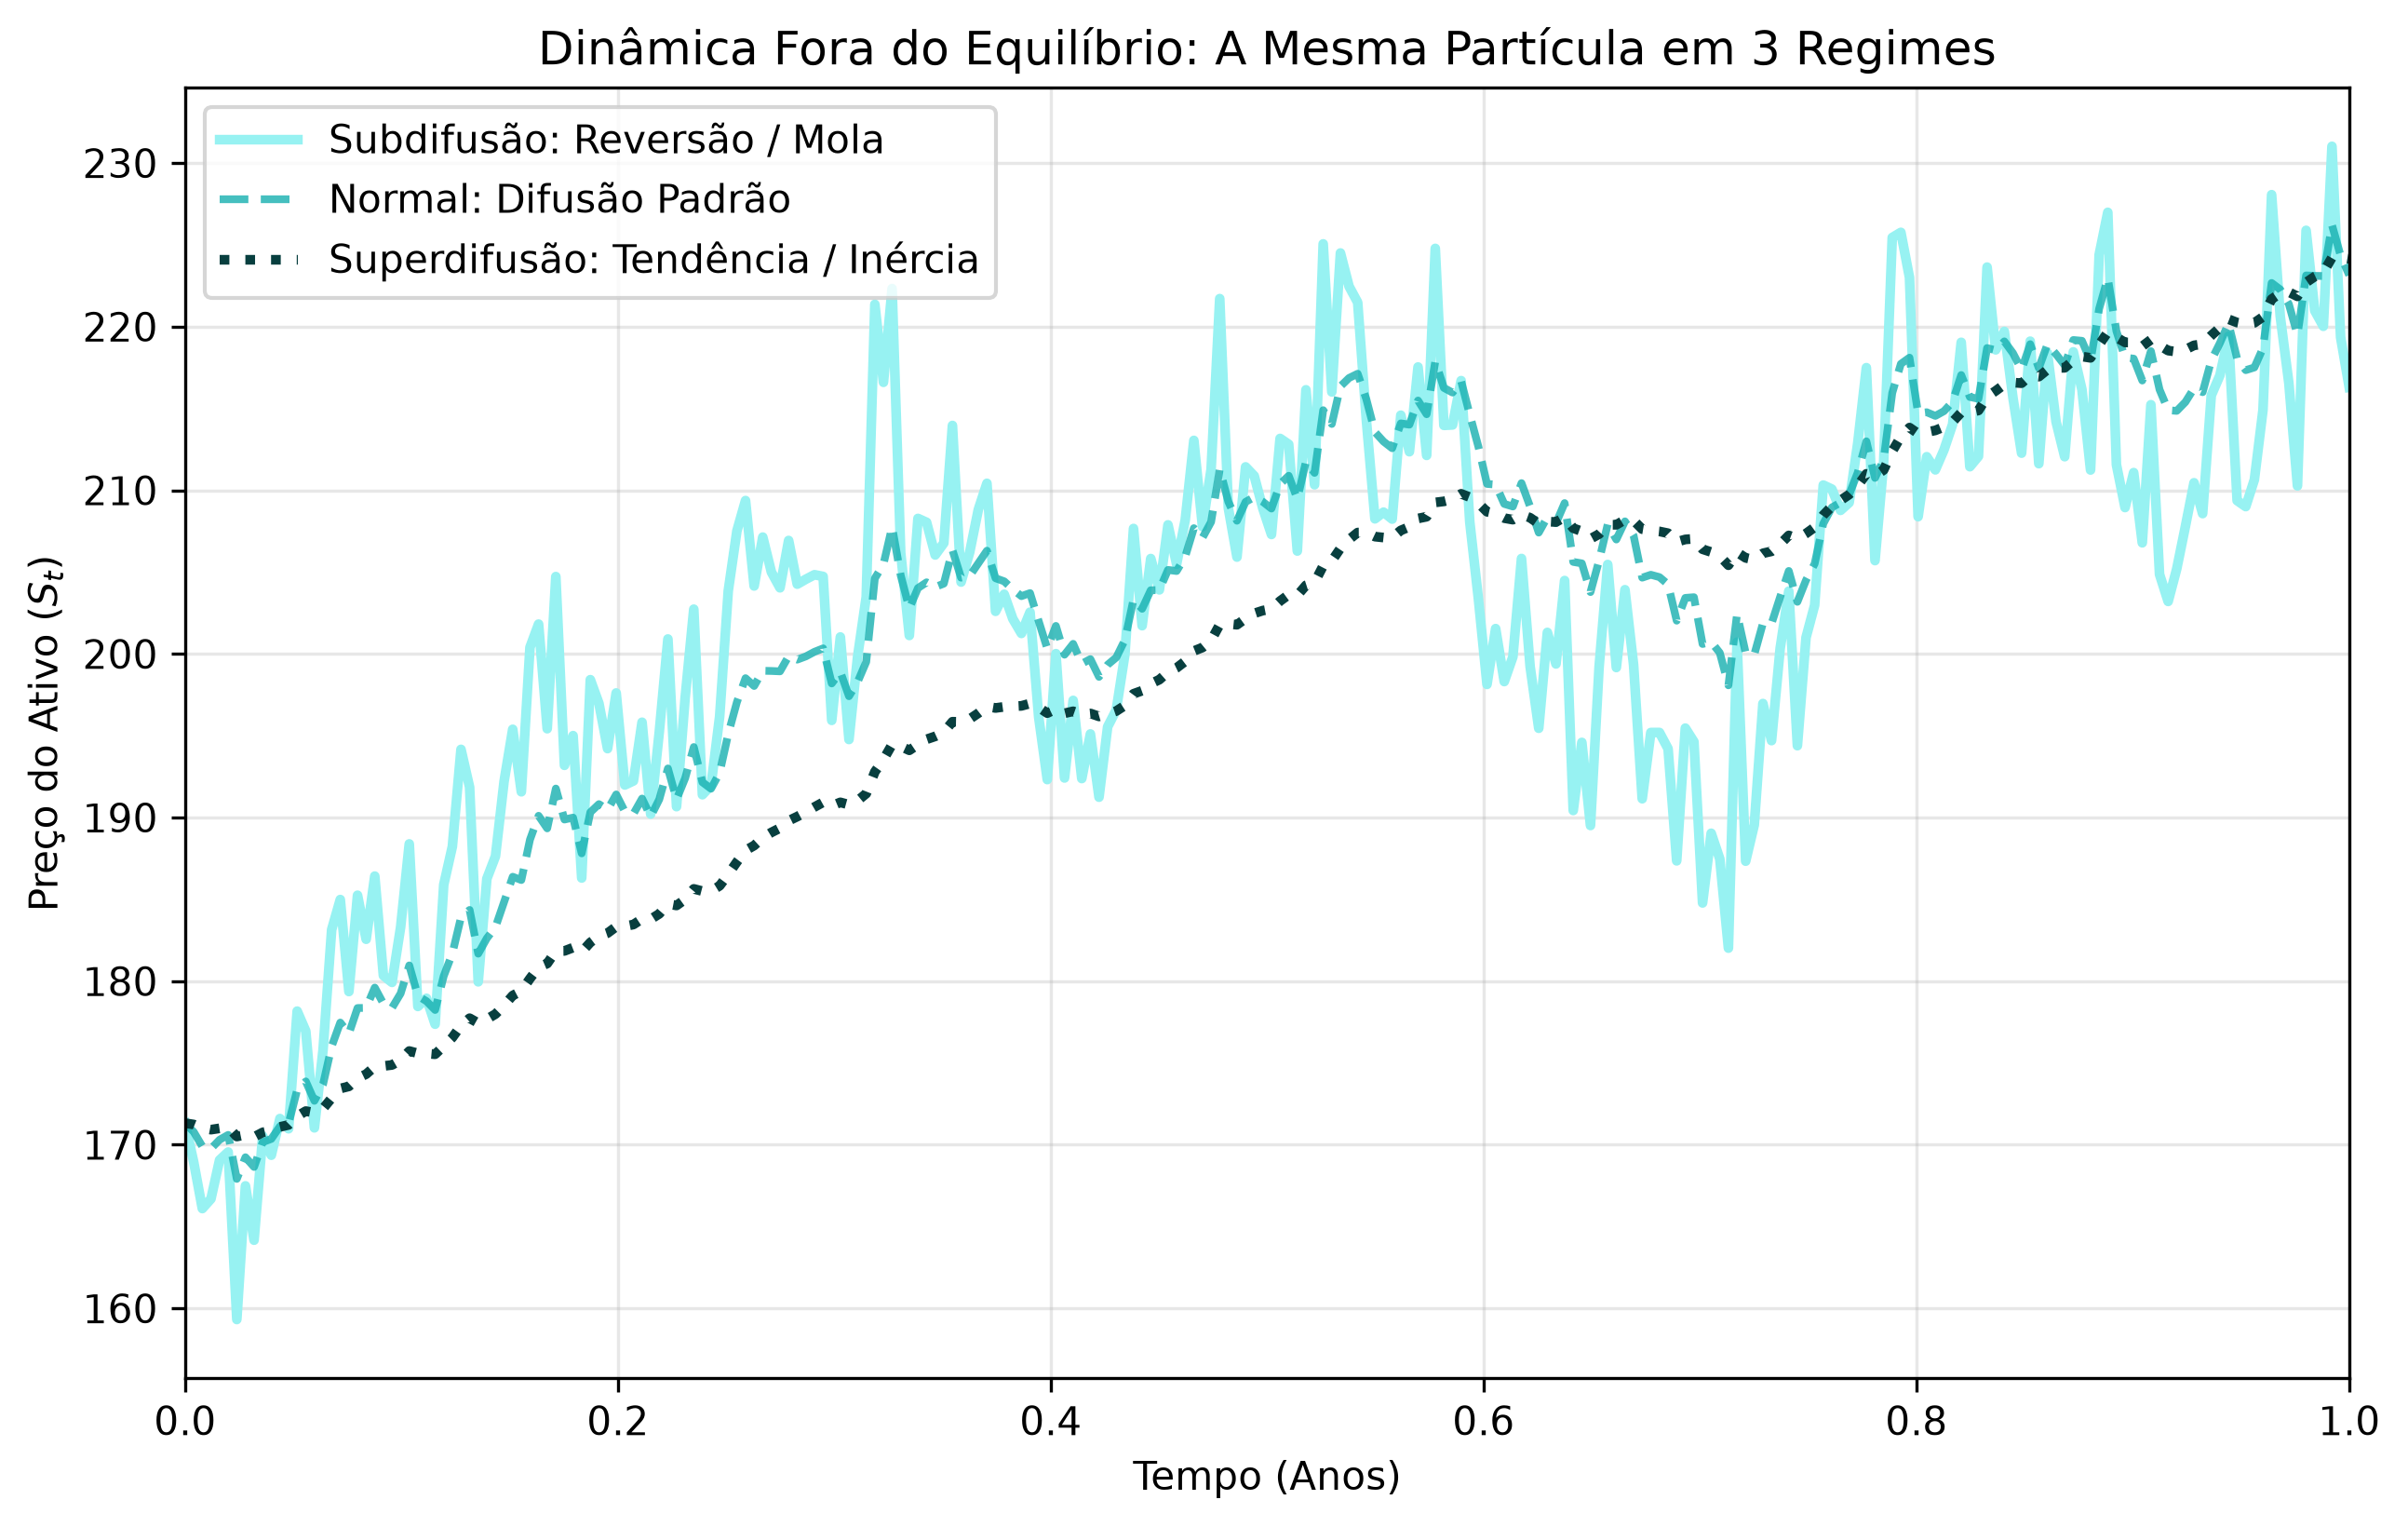
\includegraphics[width=0.85\textwidth]{../Gráficos/07_difusao_fracionaria.png}
    \caption{A mesma partícula submetida a três regimes termodinâmicos distintos. A memória espacial altera drasticamente a resposta aos mesmos choques térmicos.}
    \label{fig:trajetorias}
\end{figure}

\subsection{Assinatura Espacial: Deslocamento Quadrático Médio (MSD)}
Para validar matematicamente esta dinâmica fora do equilíbrio, isolou-se a componente puramente estocástica (removendo a força $\mu$) para analisar o Deslocamento Quadrático Médio ($\langle x^2(t) \rangle$). A dispersão teórica dita que $\text{MSD} \propto t^{2H}$. 

\begin{figure}
    \centering
    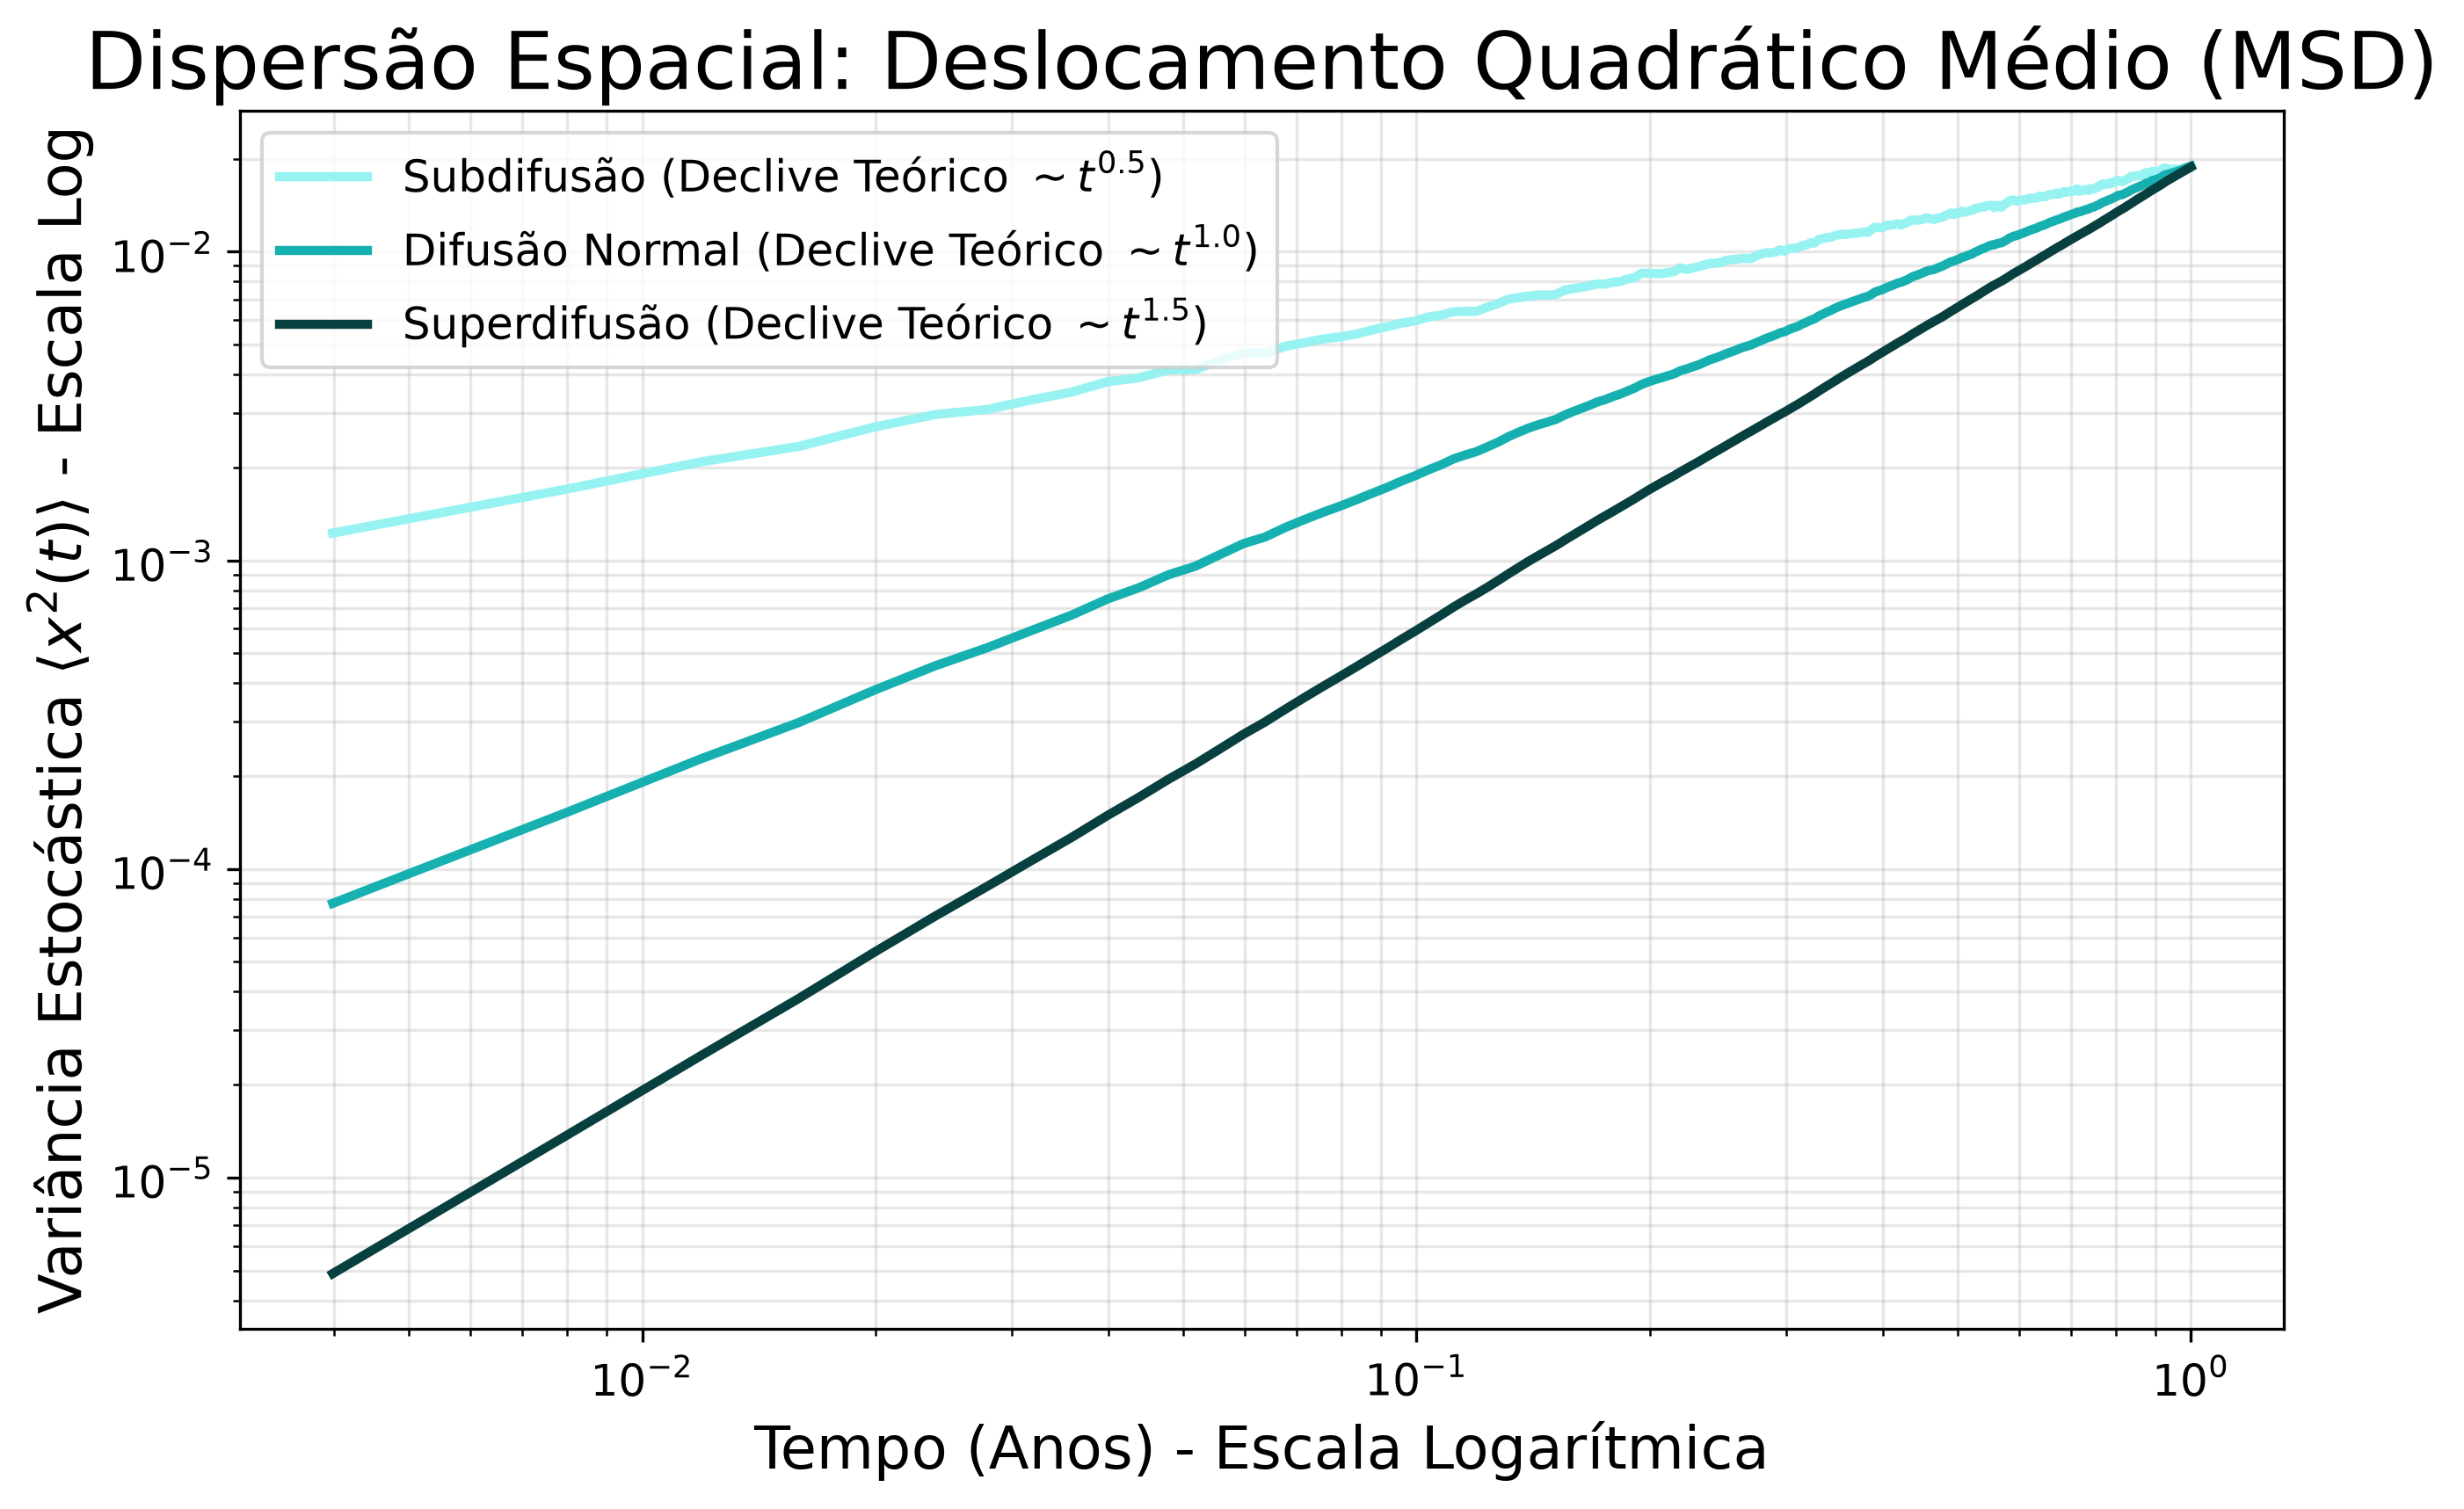
\includegraphics[width=0.85\textwidth]{../Gráficos/10_deslocamento_quadratico_medio.png}
    \caption{Evolução do Deslocamento Quadrático Médio em escala log-log. A divergência dos declives atesta a deformação do espaço provocada pelas dimensões fractais.}
    \label{fig:msd}
\end{figure}

Conforme ilustrado na Figura \ref{fig:msd}, comprovou-se que o limite de difusão normal obedece à métrica de Einstein (crescimento linear), enquanto os estados anómalos exibem leis de potência divergentes. A autocorrelação do ruído a um passo temporal (\textit{lag-1}) confirmou a propriedade elástica no espaço subdifusivo (Figura \ref{fig:autocorr}), registando um valor negativo de aproximadamente $-0.29$.

\begin{figure}
    \centering
    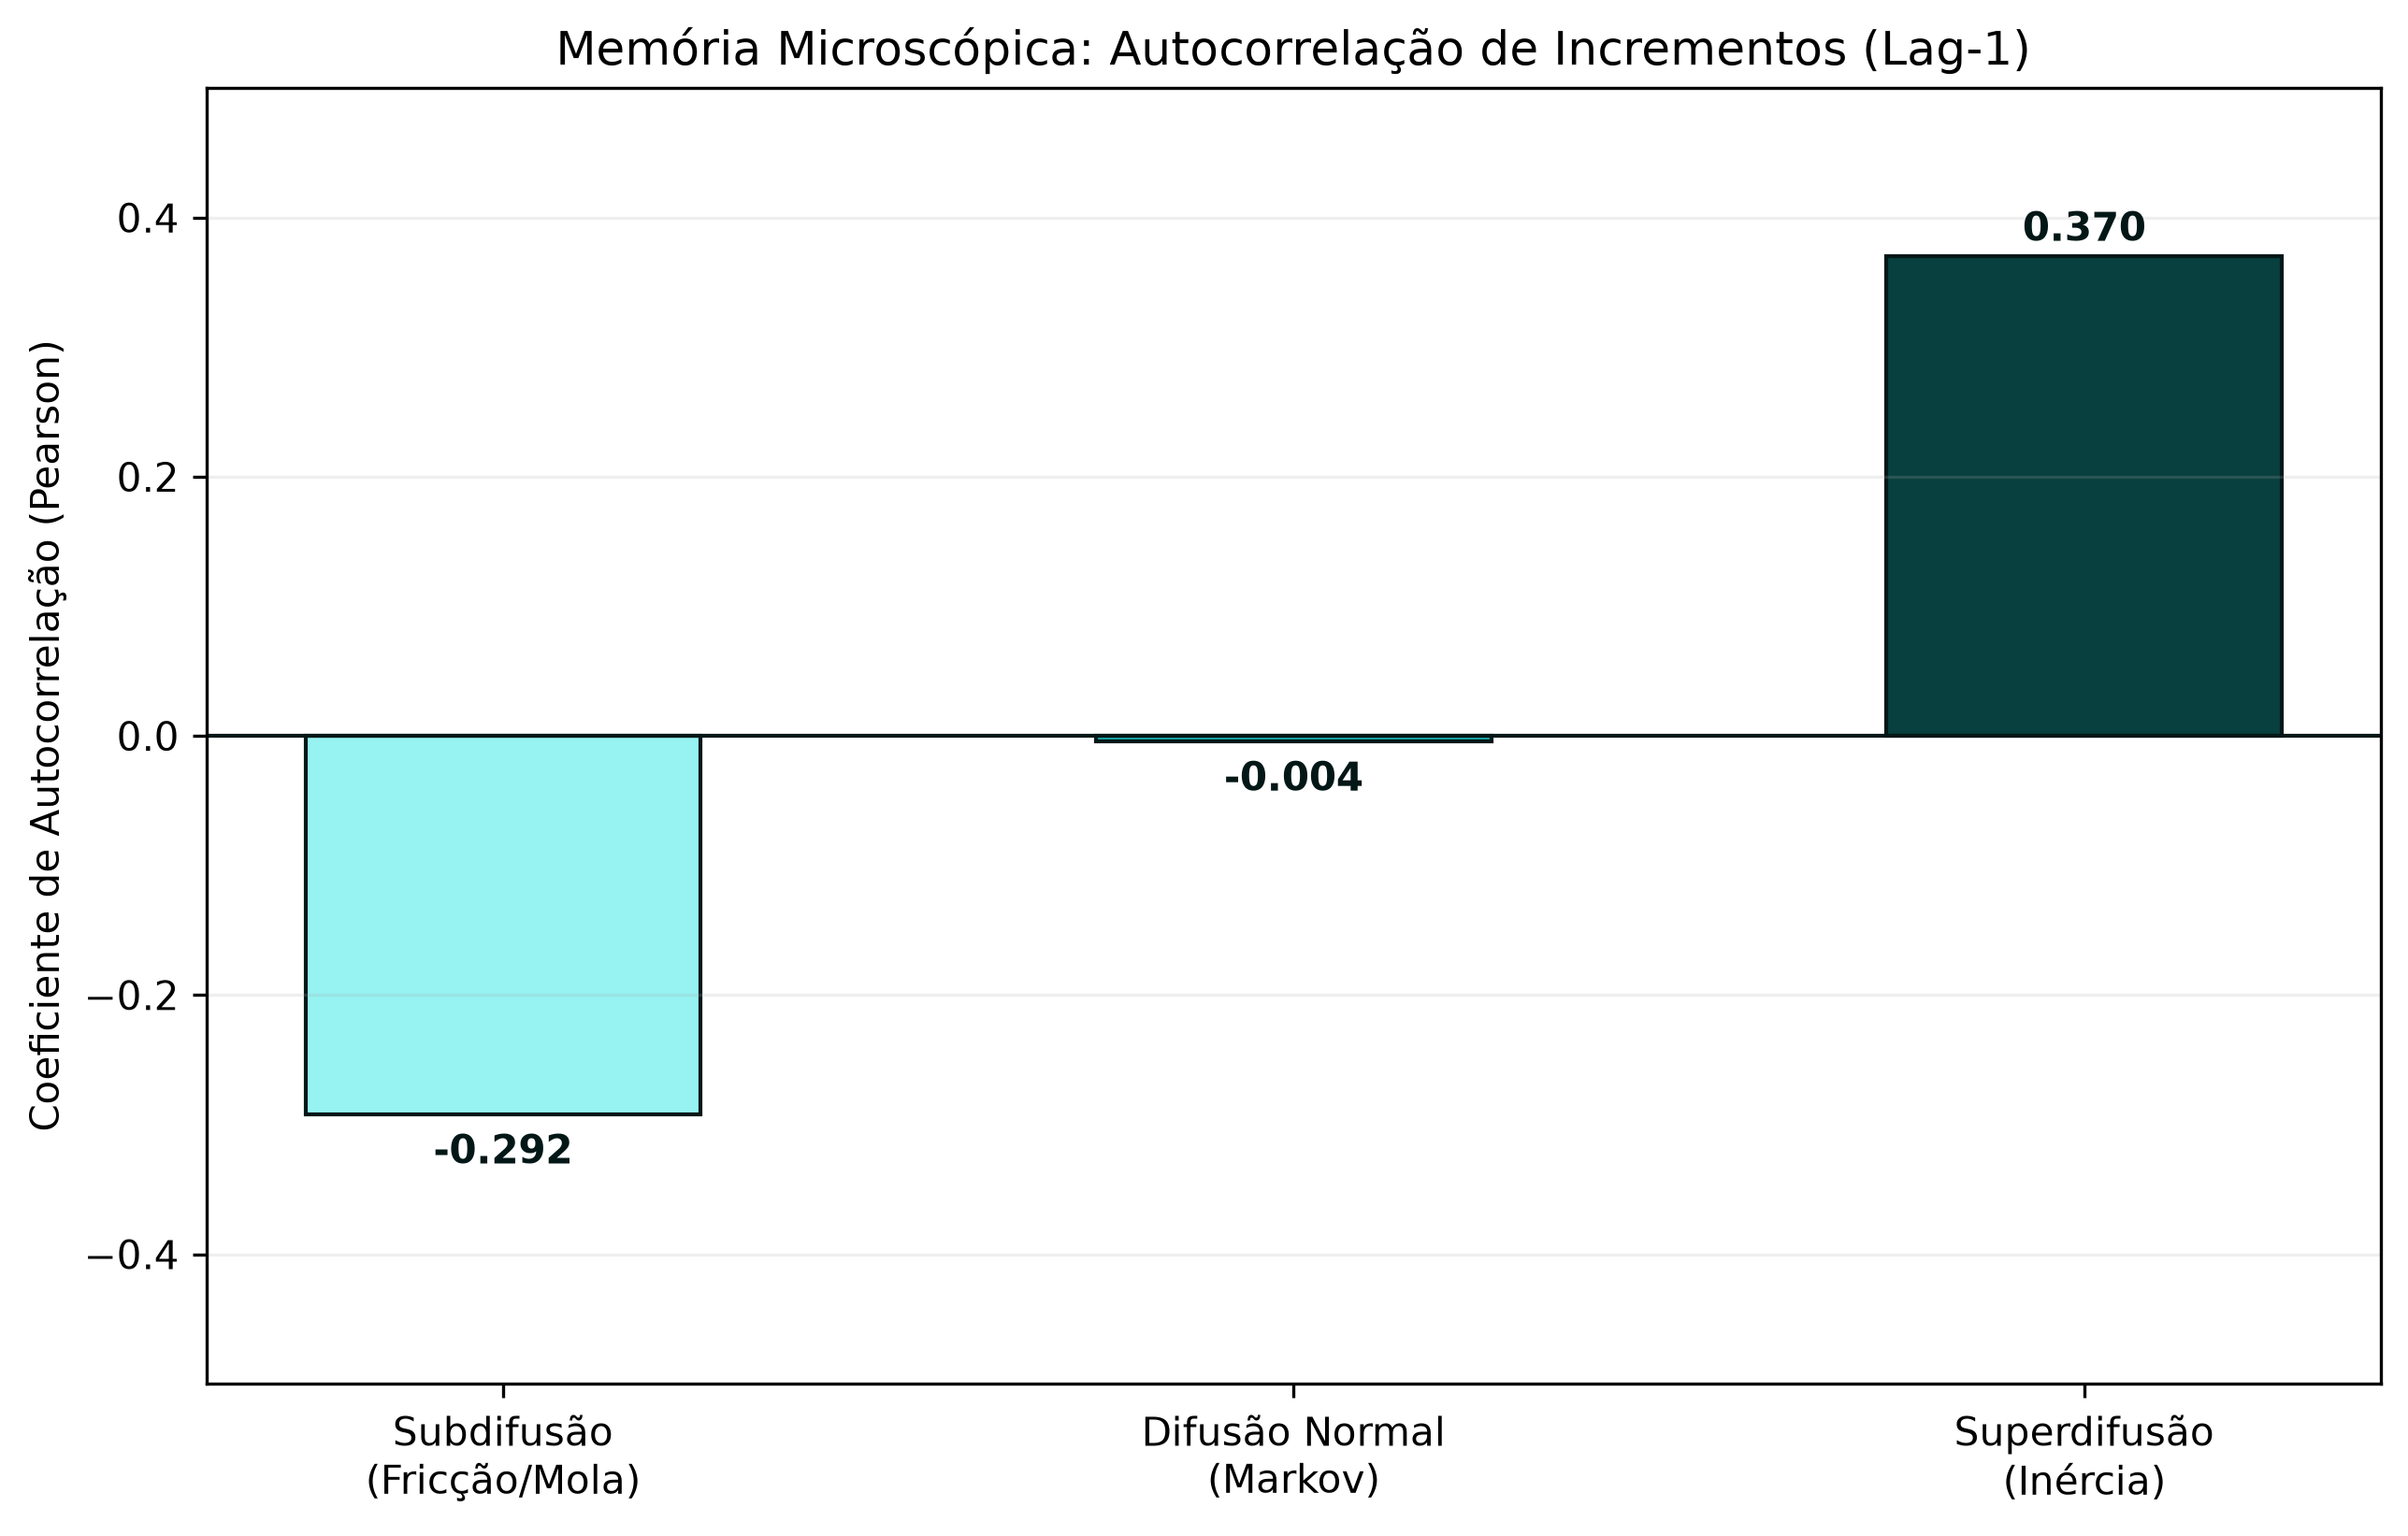
\includegraphics[width=0.7\textwidth]{../Gráficos/11_autocorrelacao_microestados.png}
    \caption{Função de autocorrelação lag-1 para os microestados dos três regimes espaciais.}
    \label{fig:autocorr}
\end{figure}

\subsection{O Problema de Fuga de Kramers (Estados Absorventes)}
Em mecânica estatística, a Taxa de Escape de Kramers define a probabilidade de uma partícula superar uma barreira de potencial devido à agitação térmica. Foram definidos dois limites de absorção: limite superior (+30\%) e limite inferior (-20\%).

A análise dos tempos de primeira passagem (Figura \ref{fig:kramers}) ditou que o regime de alta fricção (Subdifusão) destrói precocemente as partículas, apresentando a menor taxa de sobrevivência do \textit{ensamble}. 

\begin{figure}
    \centering
    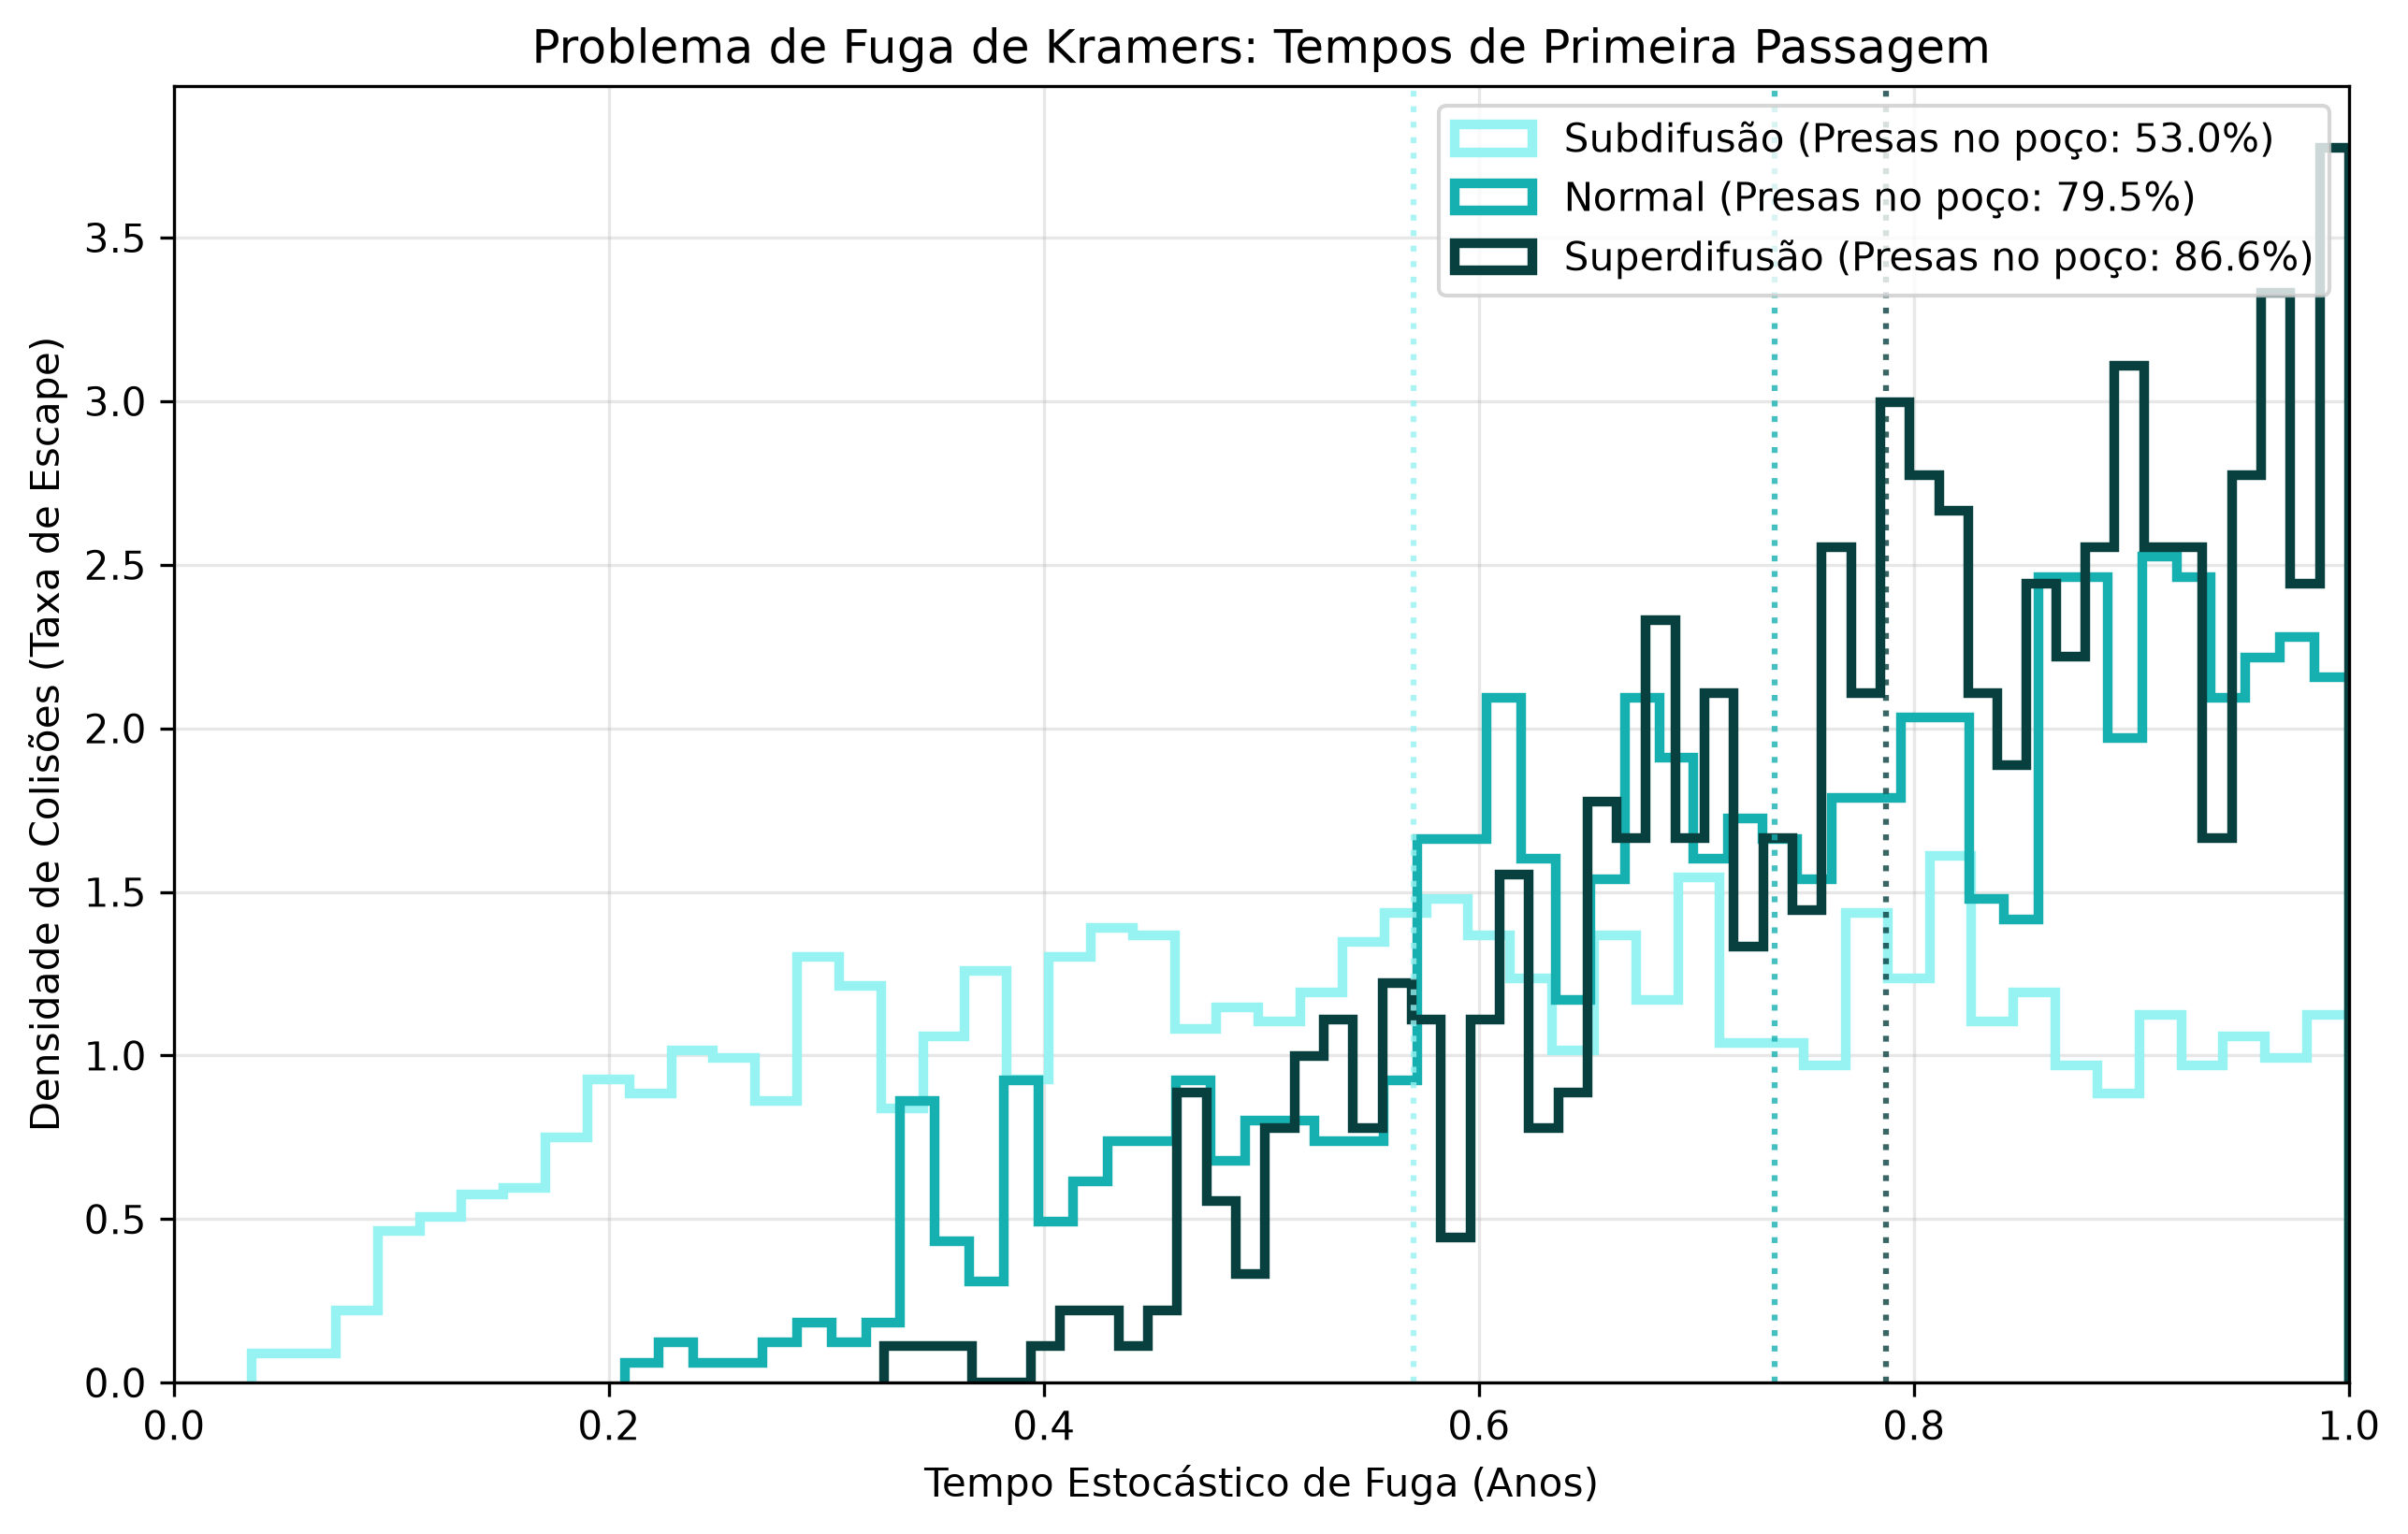
\includegraphics[width=0.85\textwidth]{../Gráficos/08_fuga_kramers.png}
    \caption{Histograma dos Tempos de Primeira Passagem simulando a Fuga de Kramers para os limites do poço de potencial termodinâmico.}
    \label{fig:kramers}
\end{figure}

A constante necessidade de manter a dispersão a curto prazo gera colisões letais com a fronteira, provando o \textbf{Paradoxo do Atrito}: a reversão à média mitiga grandes desvios a longo prazo (propriedade intrínseca à subdifusão \cite{metzler2014}), mas fá-lo exigindo choques térmicos violentos intra-anuais, maximizando o risco estatístico diário. Por outro lado, a Superdifusão apresenta uma inércia direcional amortecedora, retendo a vasta maioria das partículas no poço de potencial durante o horizonte temporal.

\subsection{A Seta do Tempo e Entropia de Shannon}
Na formulação de base da disciplina \cite{sebenta}, a entropia estatística generalizada para uma variável aleatória com distribuição de probabilidade $p(x)$ é definida como $S = - \sum p(x) \ln p(x)$. Seguindo este pressuposto e estendendo-o à quantificação da informação estatística dos microestados, mediu-se a Entropia de Shannon temporal para a distribuição de densidade das partículas. 

A Figura \ref{fig:entropia} verifica matematicamente a "seta do tempo": um aumento monotónico da desordem do sistema à medida que a energia térmica dispersa o \textit{ensamble}. 

\begin{figure}
    \centering
    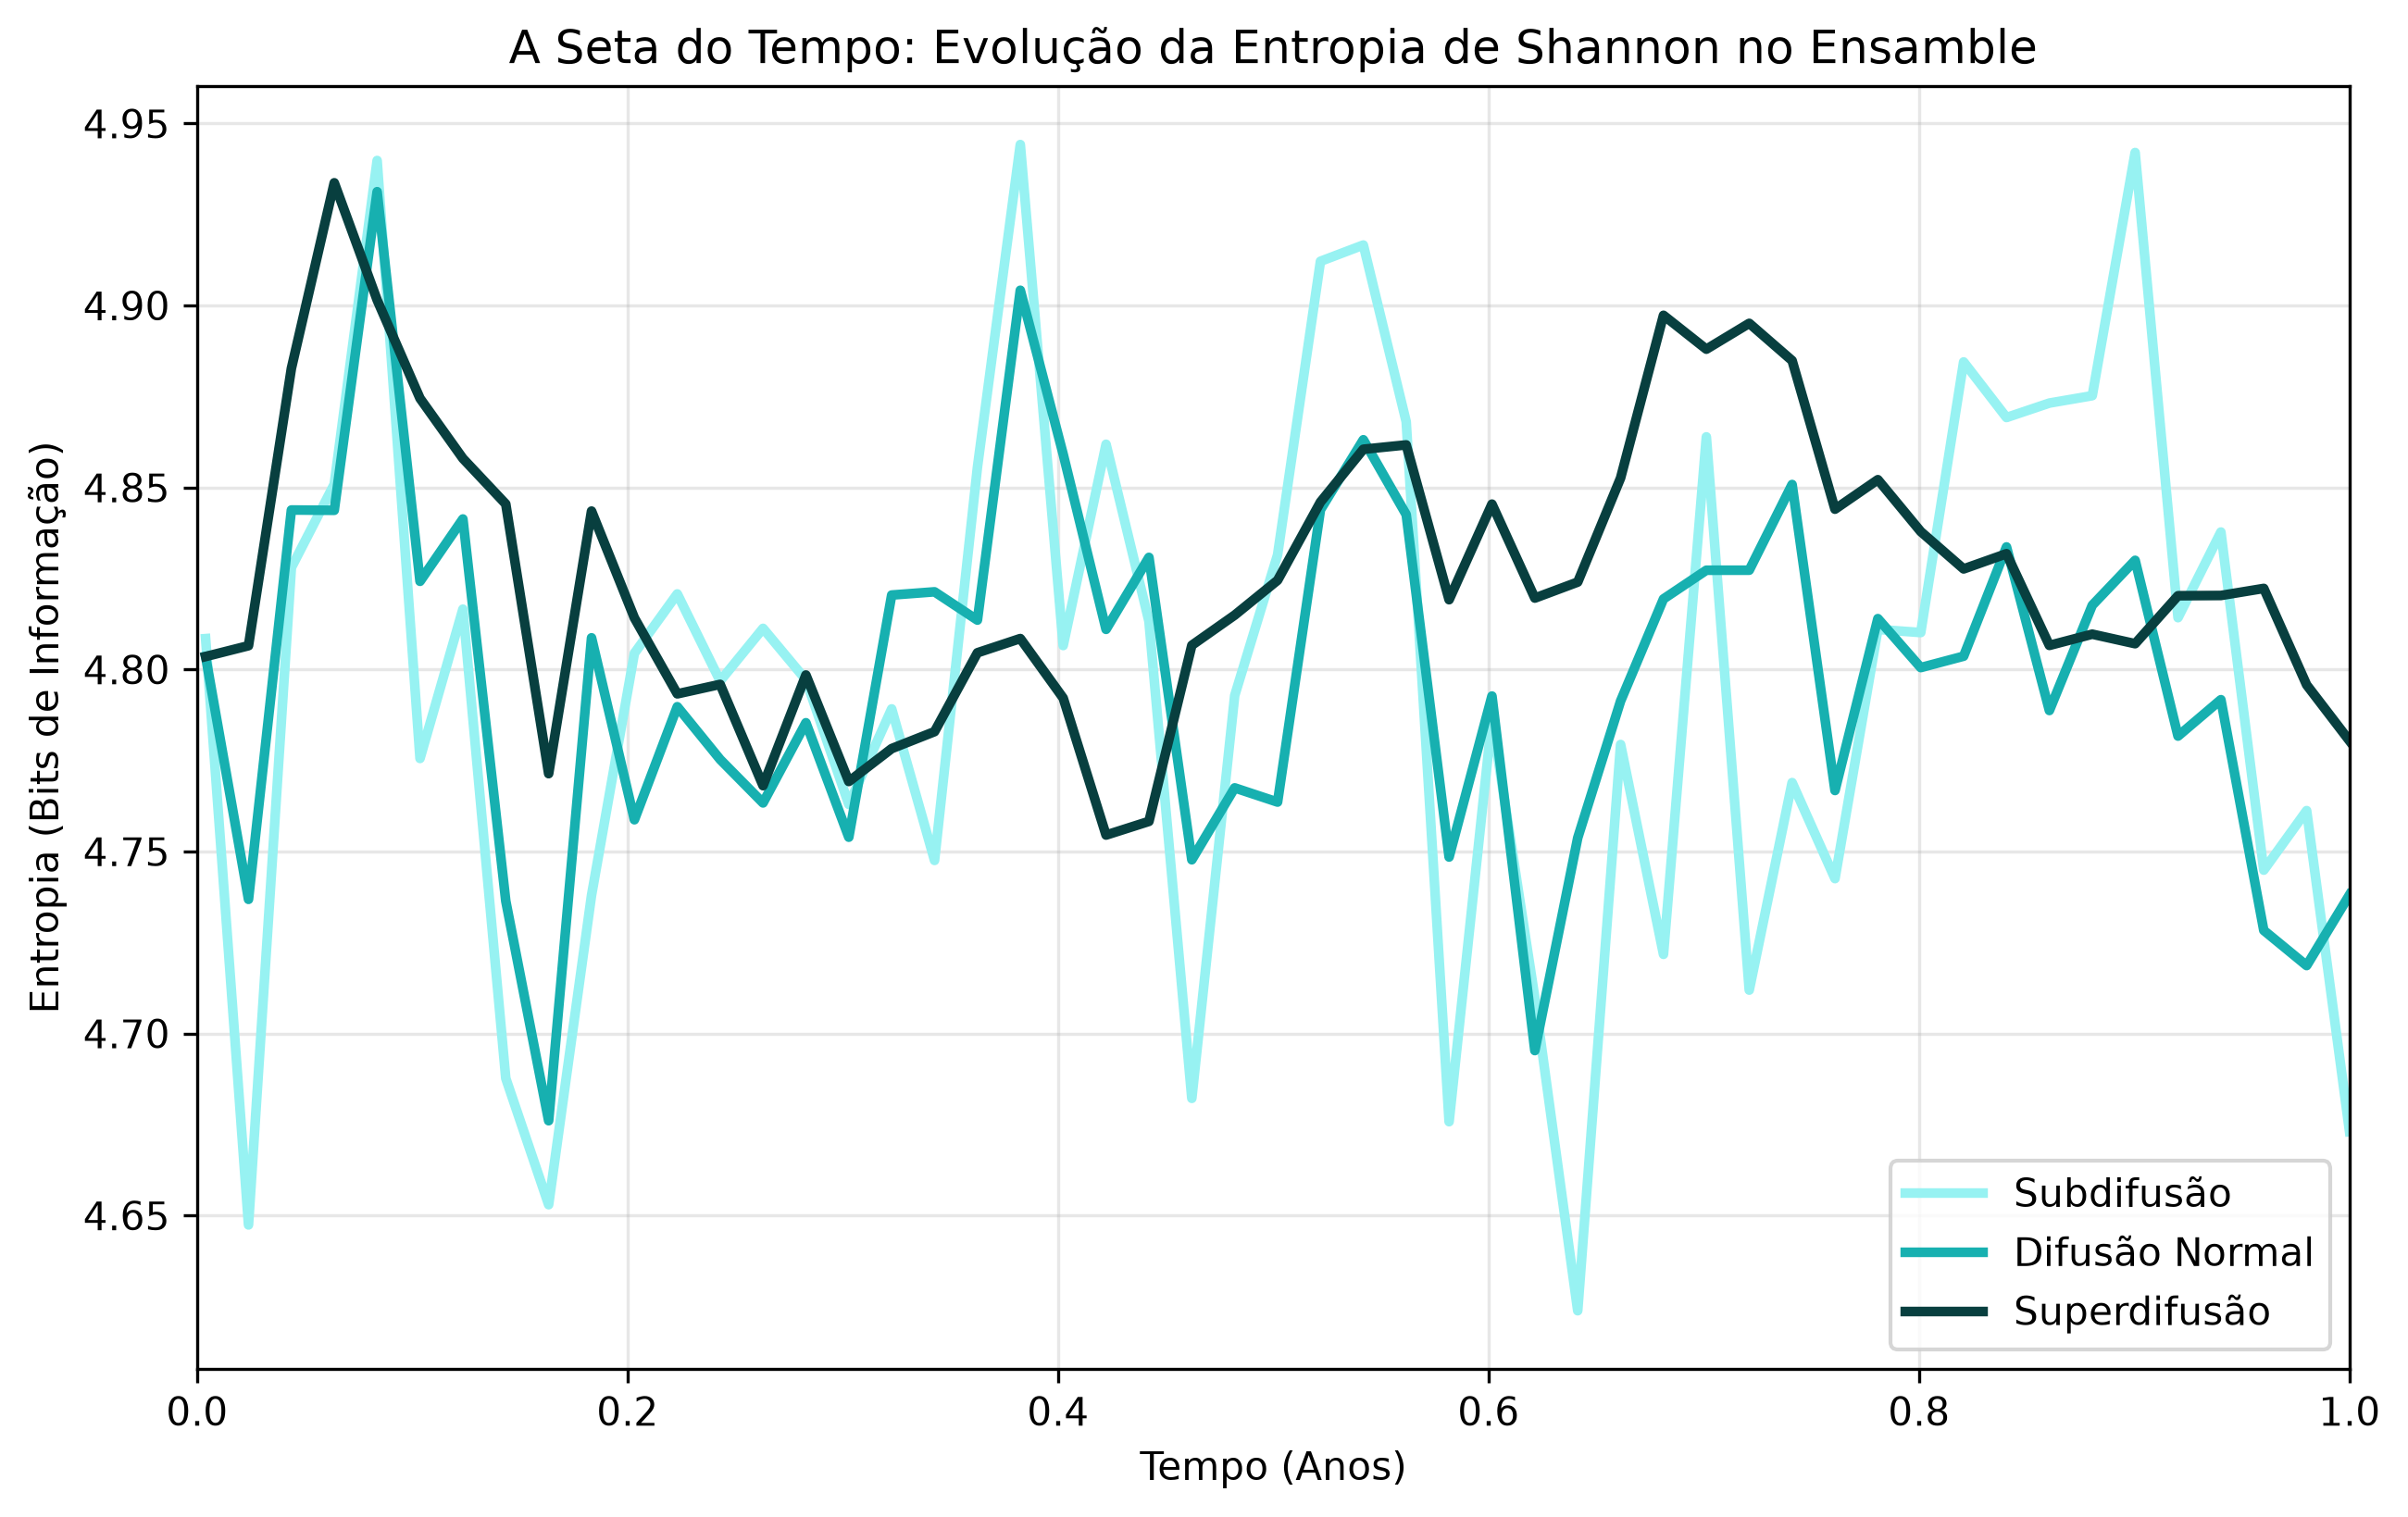
\includegraphics[width=0.85\textwidth]{../Gráficos/12_entropia_shannon.png}
    \caption{Evolução contínua da Entropia de Shannon do \textit{ensamble} de partículas ao longo do tempo.}
    \label{fig:entropia}
\end{figure}

A taxa de produção de entropia diferiu consoante a dimensão fractal, refletindo o peso relativo da dispersão ruidosa \textit{versus} a advecção estrutural da matriz.

\section{Conclusão}
A integração da Física Estatística provou que os mercados podem ser rigidamente modelados por leis da termodinâmica. A difusão anómala introduzida pelo fBM revela que a geometria e "memória" do espaço afetam drasticamente as forças de colisão macroscópicas. Modelos estritamente markovianos mascaram a perigosidade de ambientes subdifusivos e negligenciam a força da inércia superdifusiva, provando-se a necessidade de métricas como o MSD e taxas de escape de Kramers para a correta avaliação de sistemas financeiros e económicos estocásticos.

\vfill
% --- REFERÊNCIAS ---
\begin{thebibliography}{3}

\bibitem{sebenta}
Patrício, P. (2026).
\textit{Física Estatística Computacional}. Instituto Superior de Engenharia de Lisboa (ISEL).

\bibitem{metzler2014}
Metzler, R., Jeon, J.-H., Cherstvy, A.~G., \& Barkai, E. (2014).
\textit{Anomalous diffusion models and their properties: non-stationarity, non-ergodicity, and ageing at the centenary of von Smoluchowski's theory}.
Physical Chemistry Chemical Physics, 16(44), 24128--24164. \href{https://doi.org/10.1039/C4CP03465A}{DOI: 10.1039/C4CP03465A}.

\bibitem{hu2003}
Hu, Y., \& \O{}ksendal, B. (2003).
\textit{Fractional white noise calculus and applications to finance}.
Infinite Dimensional Analysis, Quantum Probability and Related Topics, 6(01), 1--32. \href{https://doi.org/10.1142/S0219025703001110}{DOI: 10.1142/S0219025703001110}.

\end{thebibliography}

\end{document}